\documentclass[a4paper,12pt]{exam}
	\usepackage{graphicx}
	\usepackage[utf8]{inputenc}
	\usepackage[T1]{fontenc}
	\usepackage{listings}
	\usepackage{color}
	\usepackage{amsmath}
	\usepackage{enumerate}
	\usepackage{caption}
	\usepackage{subcaption}
	\definecolor{dkgreen}{rgb}{0,0.6,0}
	\definecolor{gray}{rgb}{0.5,0.5,0.5}
	\definecolor{mauve}{rgb}{0.58,0,0.82}

	\lstset{frame=tb,
	  language=Python,
	  aboveskip=3mm,
	  belowskip=3mm,
	  showstringspaces=false,
	  columns=flexible,
	  basicstyle={\small\ttfamily},
	  numbers=none,
	  numberstyle=\tiny\color{gray},
	  keywordstyle=\color{blue},
	  commentstyle=\color{dkgreen},
	  stringstyle=\color{mauve},
	  breaklines=true,
	  breakatwhitespace=true
	  tabsize=3
	}

\begin{document}
\begingroup 
	  \bf \Large Mecânica Clássica I\\
	  \indent \normalsize André Del Bianco Giuffrida
	\endgroup
	\\ \quad
	\\
	O perigeu do Explorer I era de $360 km$ e o apogeu de $2549 km$ acima da superficie da terra. determine a distância da terra quando $\theta = 90^o$ onde $\theta$ é contado a partir do perigeu.
	Despresando qualquer efeito externo (Lua, Sol ou Outros planetas) vamos fazer o Explorer orbitando a terra assim como a terra orbita o sol, ou seja com a terra em um dos focos.
	Já está implícito que a órbita é fechada e elíptica e com isso partimos da equação da elipse em coordenadas polares:
	\[ r = \frac{ a(1-\epsilon^2) }{ 1+ \epsilon\cos{(\theta)} }\]
	e aqui já temos $a = d_{apogeu}+R_{terra} + $ só falta encontrar $\epsilon$
	sendo a excentricidade $\epsilon$ dada por $e = \frac{c}{a}$ onde $c$ é a distância de qualquer foco até o centro. sabemos que $c = a - p$ onde $p$ é a distância do perigeu e assim podemos plotar a orbita como segue no codigo abaixo:
		\begin{figure}[h]
			\centering
			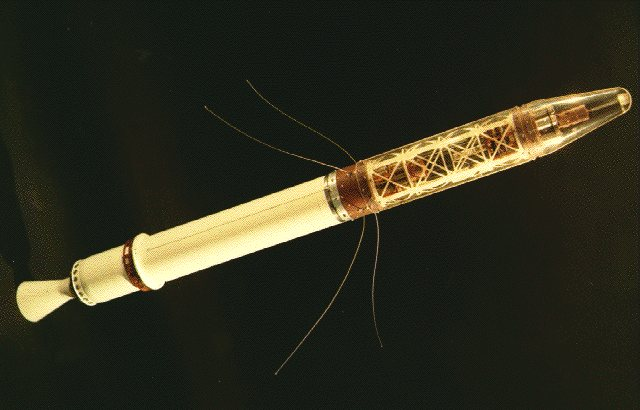
\includegraphics[scale=0.3]{Explorer1.jpg}
			\caption{Explorer I}
		\end{figure}
		\begin{lstlisting}	
		from math import *

		pi = 3.14158
		Max = 2*pi
		Resol = 0.01
		Rt = 6378
		##todas as medidas em km

		Pe = 360+Rt #Perigeu
		Ap = 2549+Rt #Apogeu

		#Foco na origem e coordenadas polares

		a = float(Pe+Ap)/2 # metade do semi-eixo maior

		c = a - float(Pe)
		e = float(c)/float(a)
		#print a,c,e
		#>> 7832.5 1094.5 0.139738270029
		for i in range(0,int(Max/Resol)):
			t = float(i)*Resol
			r = a*(1-pow(e,2))/(1+ e*cos(t))
			print t,r

	\end{lstlisting}
		\begin{figure}[h]
			\centering
			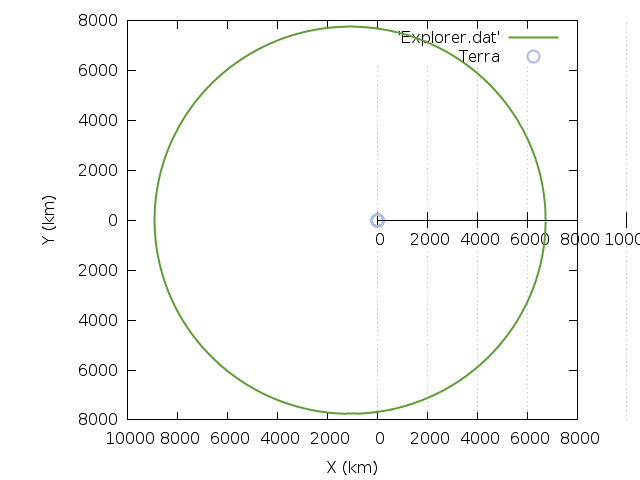
\includegraphics[scale=0.3]{5o0.png}
			\caption{Explorer I}
		\end{figure}
	\[
	\begin{array}{lll}
		a=7832.5 km \\
		c=1094.5 km \\
		e = 0.1397 \\
	\end{array}
	\]
	\[ r(\theta) = \frac{7679,64}{1+0.1397cos(\theta)} km \]
	Então para responder a pergunta :\\
	Qual a distância da superficie da terra quando $\theta = 90^o$ basta avaliar a equação de modo que:
	\[r(\pi/2) =  7679,64 km \quad \text{do centro,} \]
	\[r - R_t = (7679,64 - 6378 )km = 1301,64 km\] 
	Ou seja, a Explorer ficava a $1301,64 km$ da superfície da terra quando $\theta = 90^o$

	\end{document}
